\section{Réalisation de l'application}
\paragraph{}
Ici, nous faisons part de captures d'écran des différentes fonctionnallités de l'application. \par 

\begin{figure}[h]
        \centering
        
\includegraphics[width=1\textwidth]{accueil}
        \caption{Accueil}
        \label{image-accueil}
\end{figure}

\begin{figure}[h]
        \centering
        
\includegraphics[width=1\textwidth]{a_propos}
        \caption{A propos}
        \label{image-a_propos}
\end{figure}

\begin{figure}[h]
        \centering
        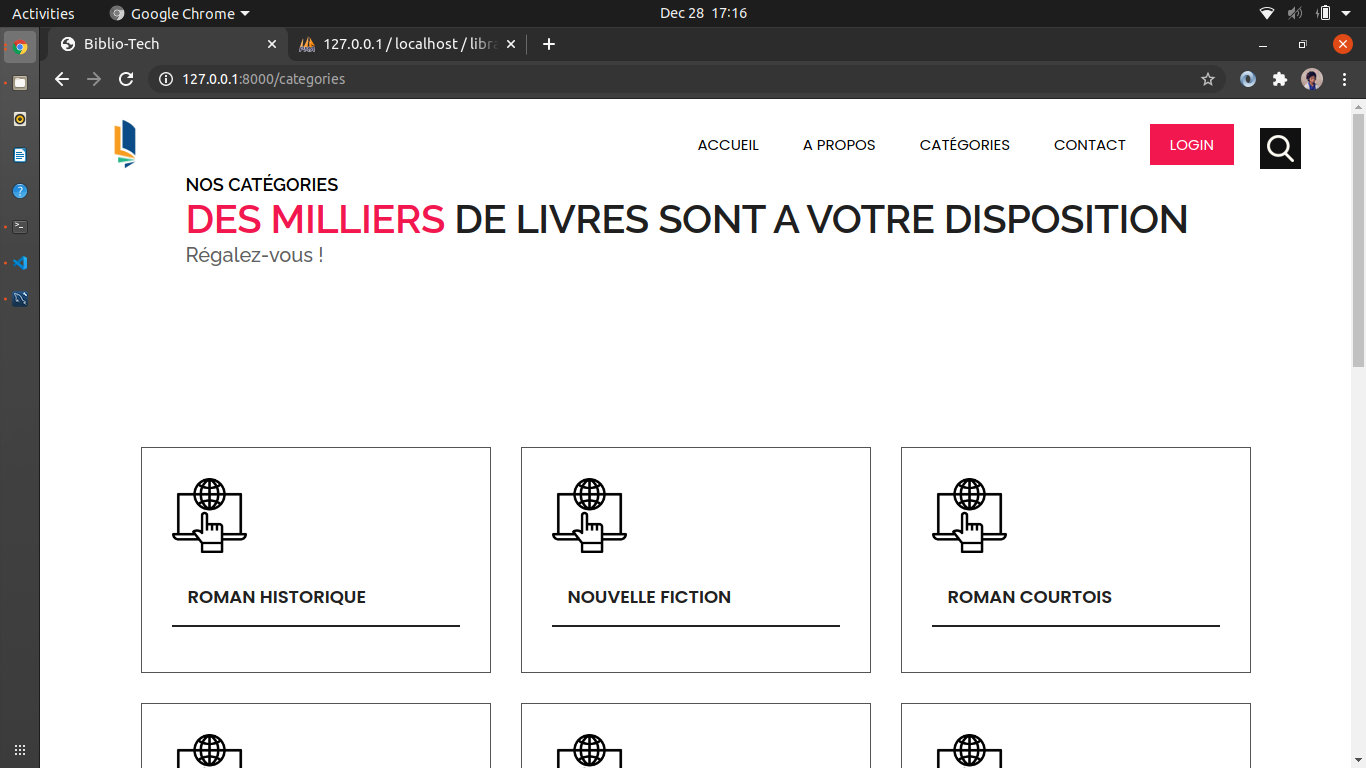
\includegraphics[width=1\textwidth]{categories}
        \caption{Catégories}
        \label{image-categories}
\end{figure}

\begin{figure}[h]
        \centering
        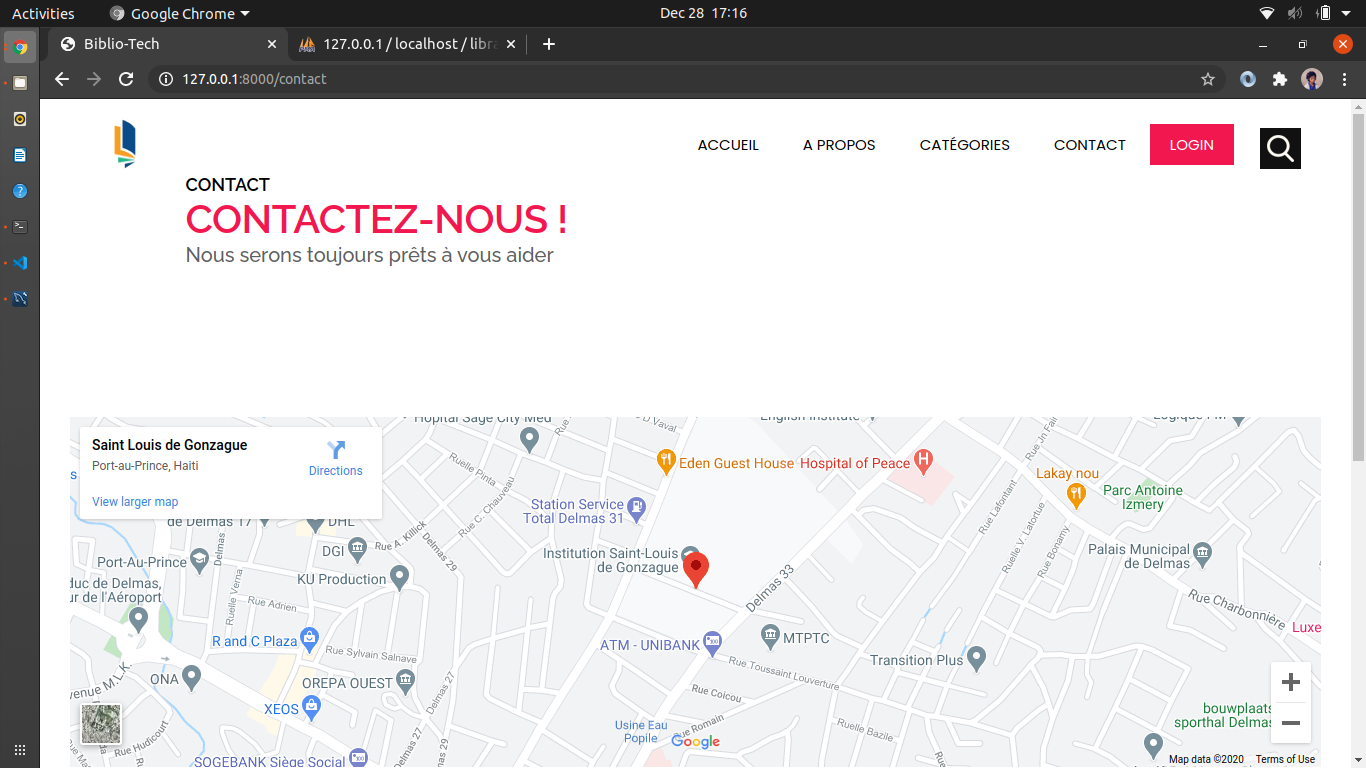
\includegraphics[width=1\textwidth]{contact}
        \caption{Contact}
        \label{image-contact}
\end{figure}

\begin{figure}[h]
        \centering
        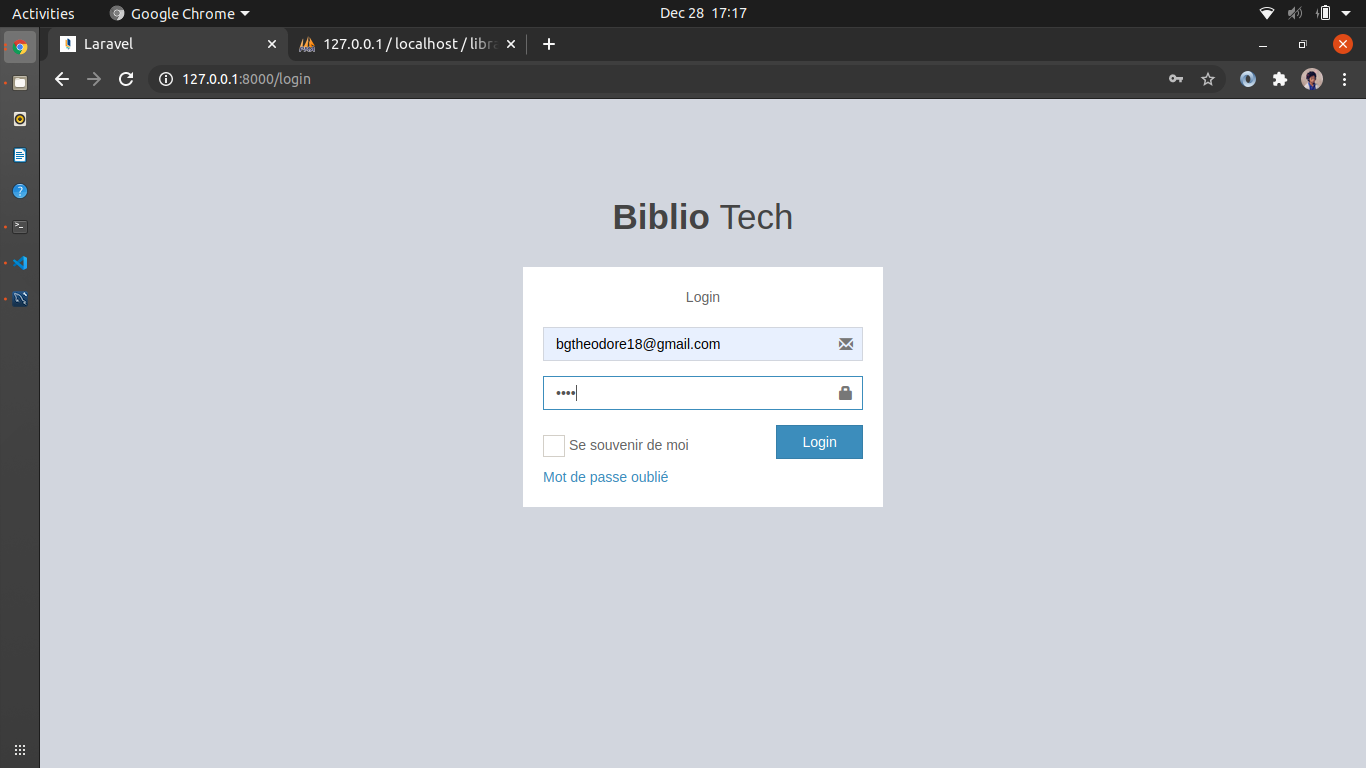
\includegraphics[width=1\textwidth]{login}
        \caption{Login}
        \label{image-login}
\end{figure}

\begin{figure}[h]
    \centering
    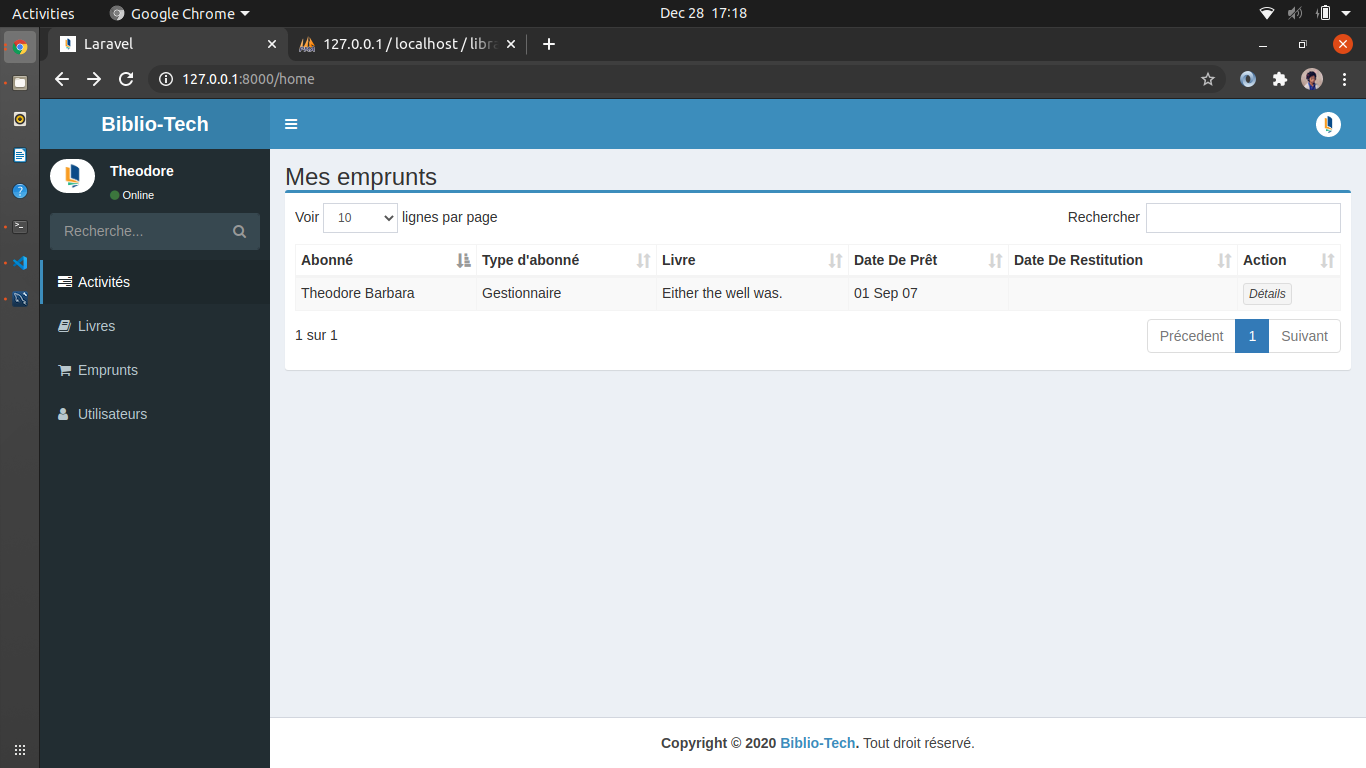
\includegraphics[width=1\textwidth]{interface_gestionnaire}
    \caption{Interface du gestionnaire}
    \label{image-interface_gestionnaire}
\end{figure}

\begin{figure}[h]
    \centering
    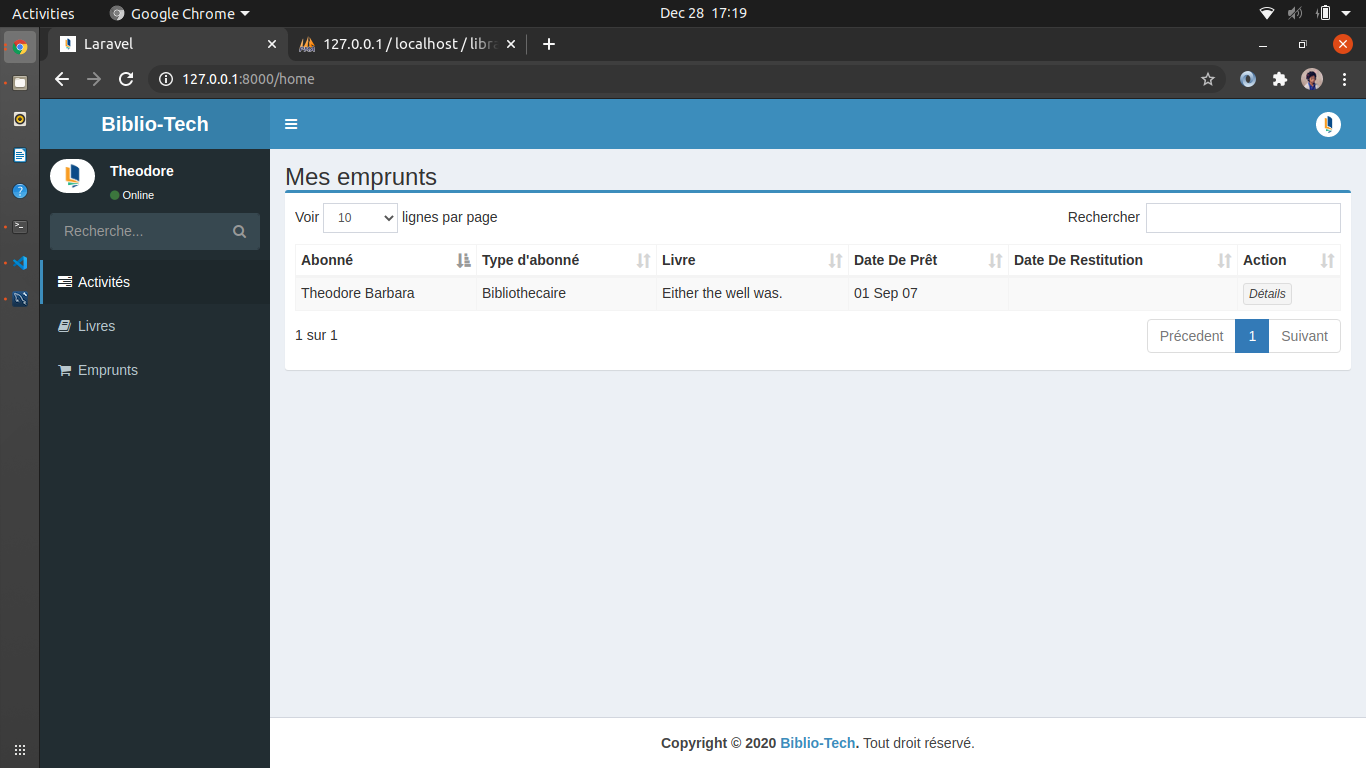
\includegraphics[width=1\textwidth]{interface_bibliothecaire}
    \caption{Interface du bibliothécaire}
    \label{image-interface_bibliothecaire}
\end{figure}

\begin{figure}[h]
    \centering
    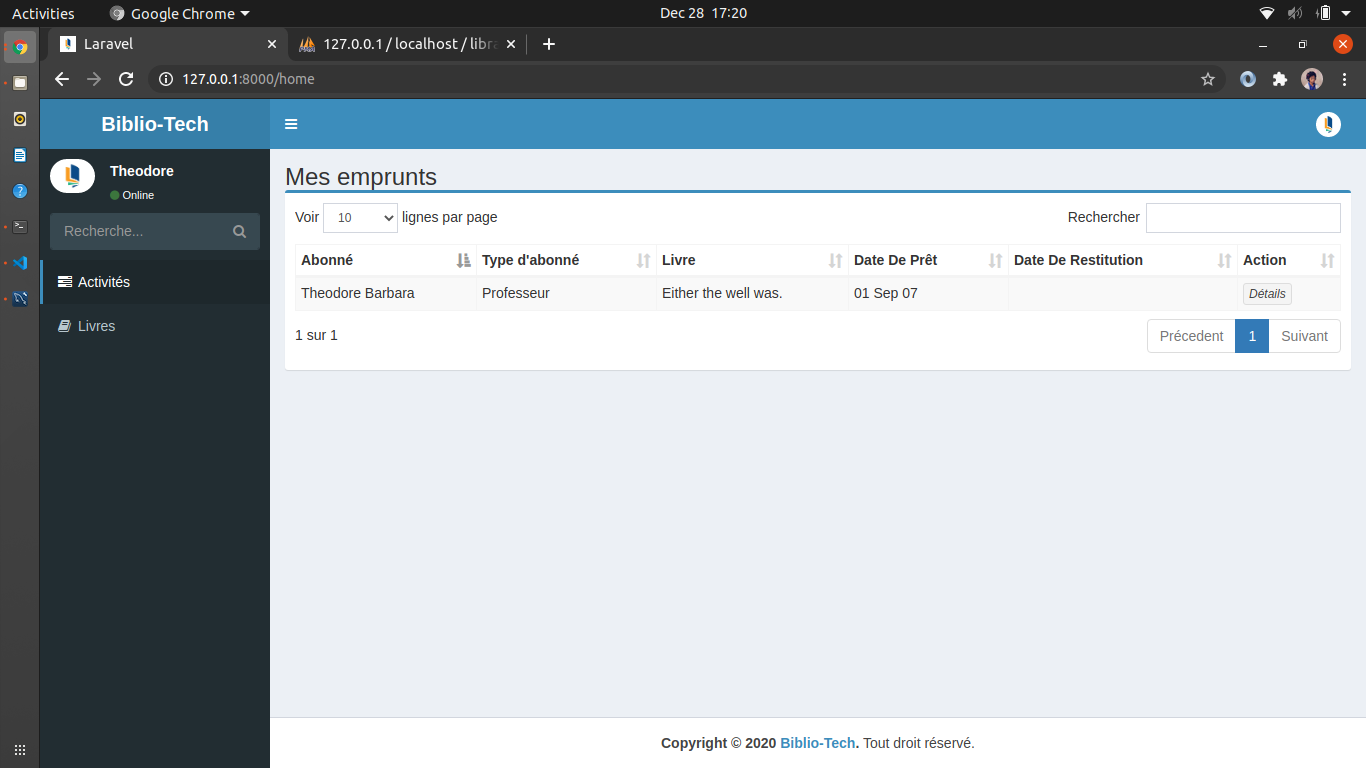
\includegraphics[width=1\textwidth]{interface_abonne}
    \caption{Interface de l'abonné}
    \label{image-interface_abonne}
\end{figure}

\begin{figure}[h]
    \centering
    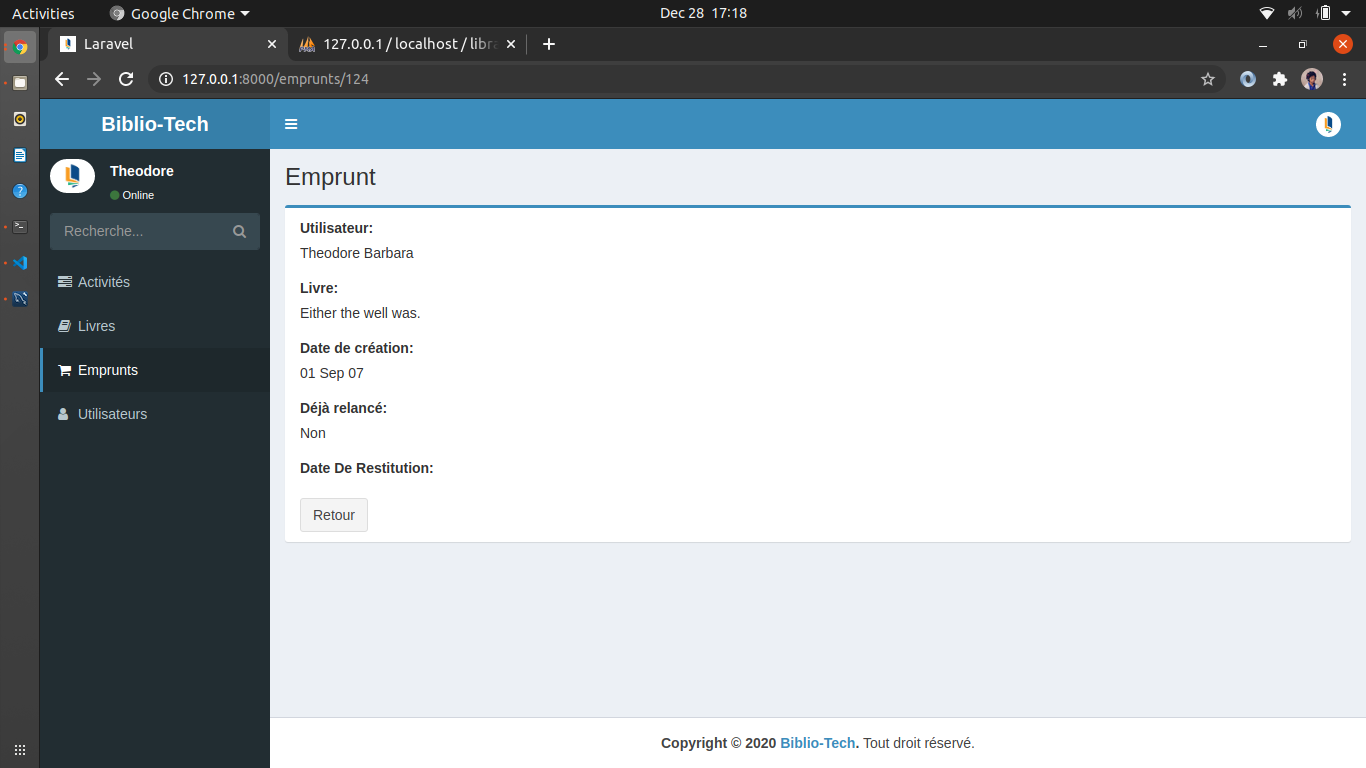
\includegraphics[width=1\textwidth]{emprunt_personnel}
    \caption{Emprunt personnel d'un utilisateur}
    \label{image-emprunt_personnel}
\end{figure}

\begin{figure}[h]
    \centering
    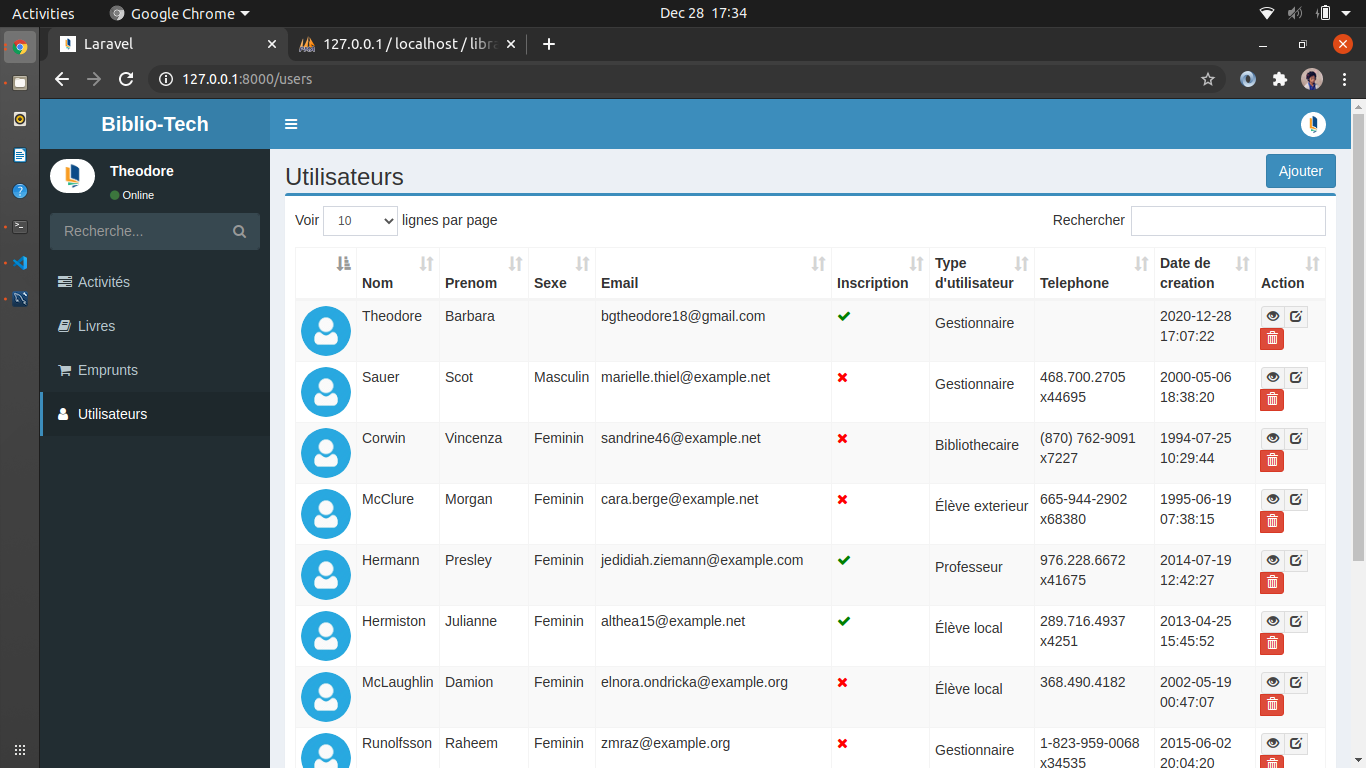
\includegraphics[width=1\textwidth]{liste_utilisateur}
    \caption{Liste des utilisateurs}
    \label{image-liste_utilisateur}
\end{figure}

\begin{figure}[h]
    \centering
    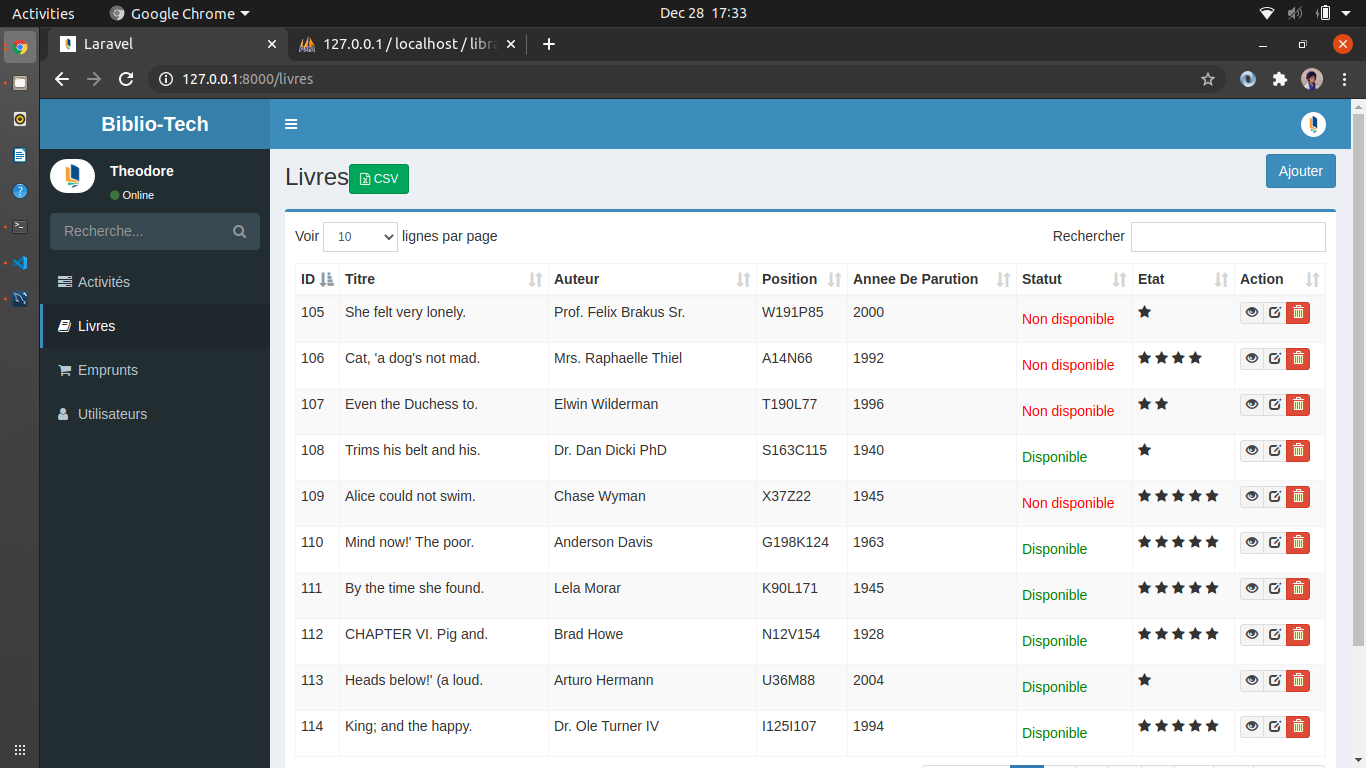
\includegraphics[width=1\textwidth]{liste_livres}
    \caption{Liste des livres}
    \label{image-liste_livres}
\end{figure}

\begin{figure}[h]
    \centering
    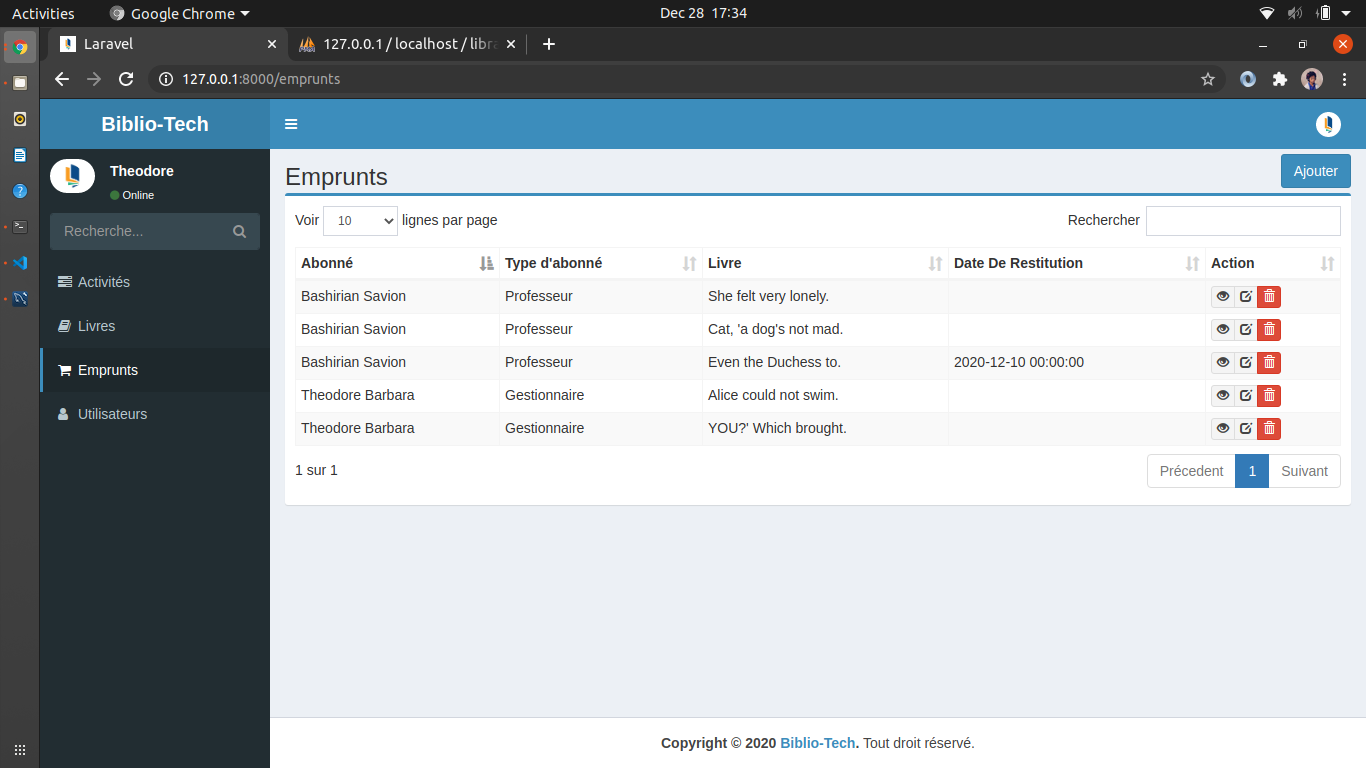
\includegraphics[width=1\textwidth]{liste_emprunt}
    \caption{liste des emprunts}
    \label{image-liste_emprunt}
\end{figure}

\begin{figure}[h]
    \centering
    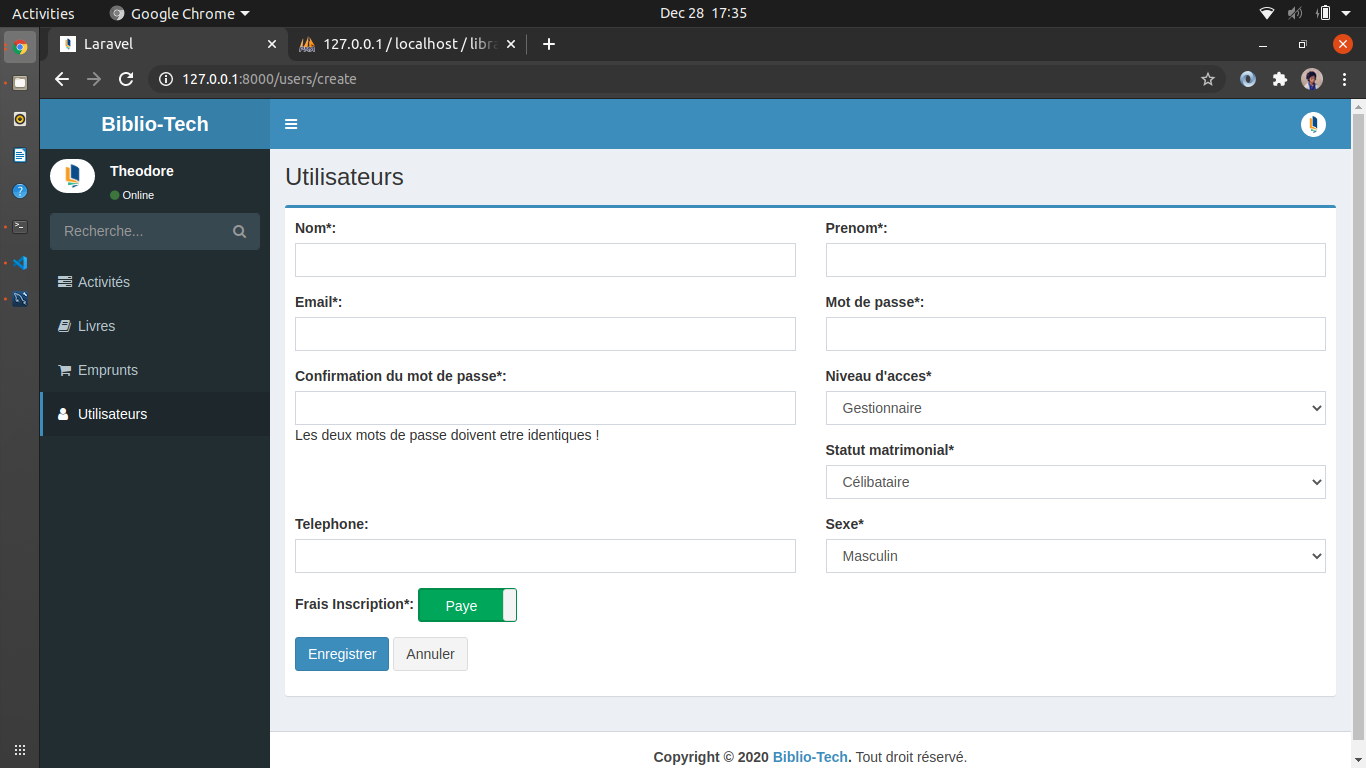
\includegraphics[width=1\textwidth]{ajout_utilisateur}
    \caption{Ajout d'un nouvel utilisateur}
    \label{image-ajout_utilisateur}
\end{figure}

\begin{figure}[h]
    \centering
    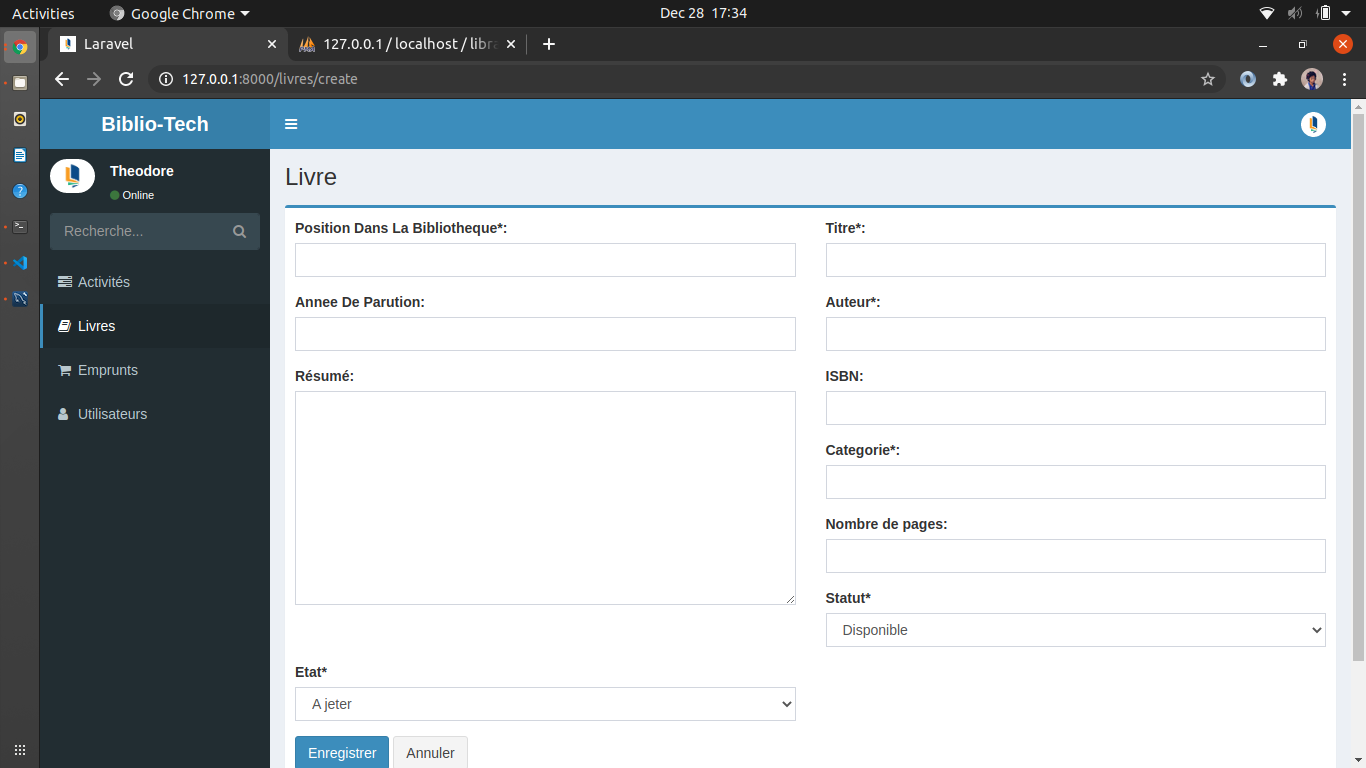
\includegraphics[width=1\textwidth]{ajout_livre}
    \caption{Ajout d'un nouveau livre}
    \label{image-ajout_livre}
\end{figure}

\begin{figure}[h]
    \centering
    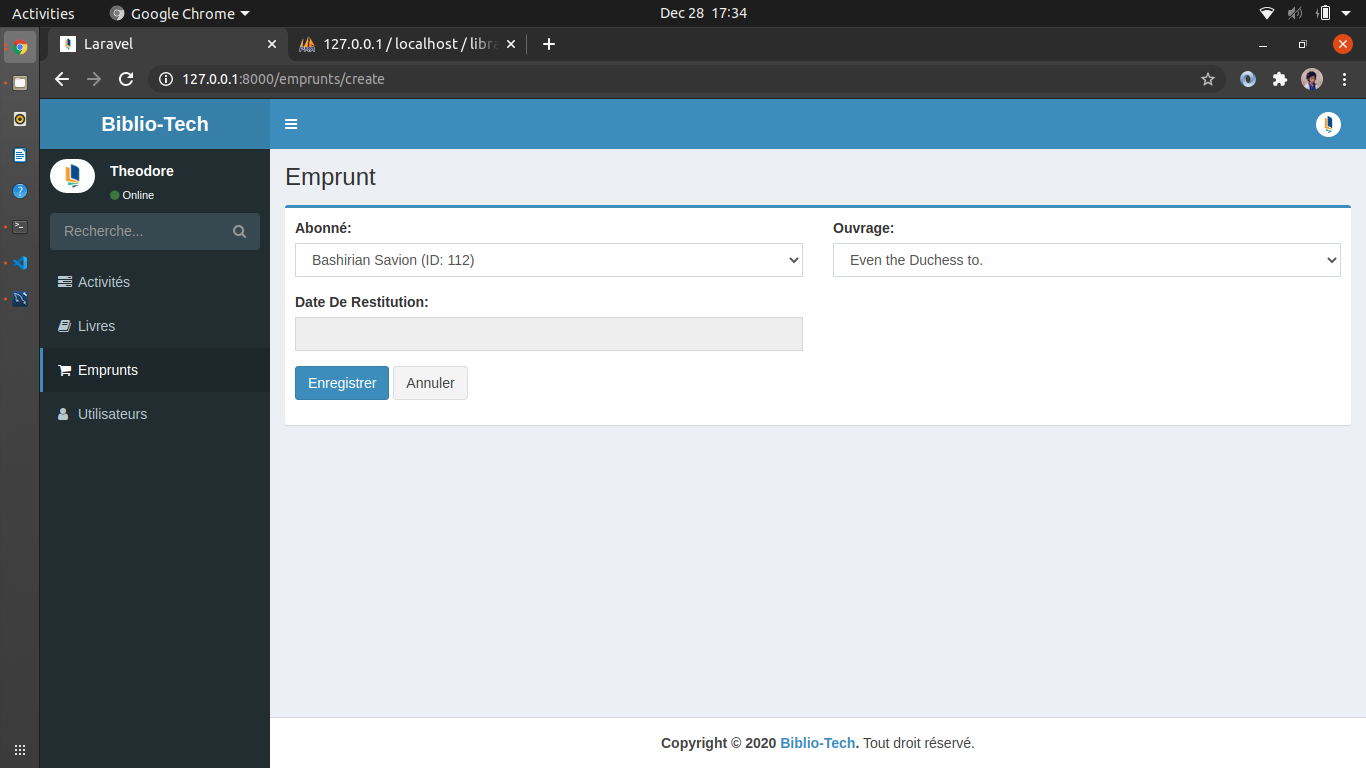
\includegraphics[width=1\textwidth]{ajout_emprunt}
    \caption{Ajout d'un nouvel emprunt}
    \label{image-ajout_emprunt}
\end{figure}